\documentclass{article}
\usepackage{listings}
\usepackage[utf8]{inputenc}
\usepackage{ amssymb }
\usepackage{amsfonts}
\usepackage{graphicx}

\title{Sistemas Distribuidos y Verificación \\ Tarea 2}
\author{Fabián Romero Jiménez}
\begin{document}
\maketitle

\begin{enumerate}

\item[\bf{Problema 1}] Considera el modelo de memoria compartida visto en clase libre de espera, y el diagrama de la Figura 1. Donde las flechas indican la especificación de la tarea $\delta$.\\

\begin{center}
  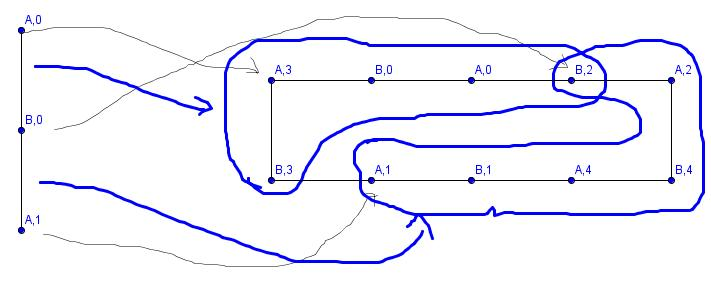
\includegraphics[width=350pt]{t2_f1.jpeg}\\
  Figura 1
\end{center}

\begin{enumerate}

\item Demuestra que existe un protocolo que puede resolver la tarea, considera que se puede ejecutar más de una lectura y escritura sobre el mismo arreglo mem[A,B].\\

  Considere el siguiente mapeo:
  
  Consideremos el camino $\{B3,A3,B0,A0,B2,A2,B4,A4,B1,A1\}$ como la únion de los caminos $\{B3,A3\} \cup \{A3,B0,A0,B2\} \cup \{B2,A2,B4,A4,B1,A1\}$
  
  En el primer turno mandamos $\{A0,B0\}$ al camino $\{A3,B0,A0,B2\}$ pues como vimos en clase sabemos que en cada turno una arista se trisecta, en el segundo turno no trisectamos y cada proceso mantiene su resolución.

  En el primer turno mandamos $\{B0,A1\}$ a un camino $\{B2,A2,B1,A1\}$ y en el segundo turno a $\{B2,A2,B2,A2,B4,A4,B1,A1,B1,A1\}$.

 Y el protocolo propuesto es una solucón de la tarea pues respeta a $\Delta$ y es un mapeo simplicial.

\item Demuestra que con un protocolo de una ronda no se puede resolver
el problema.

  Observe que $\Delta$ manda a $B0$ en $B2$ y a $A1$ en $A1$, y que en el complejo dado el camino entre esos dos vértices que está en el mapeo de la arista $\{B0,A1\}  $ es de longitud 5, es decir, en un paso tenemos que expander una arista en un camino de longitud 5, pero como vimos en clase, cada paso cuando más trisecta la arista, por lo que no es posible resolver la tarea en un paso $\blacksquare$.

\end{enumerate}


\item[\bf{Problema 2}] Sea $\delta$ un mapeo simplicial, que nos lleva de una gráfica $G$ a una gráfica $H$, $\delta$ mapea los vértices de G sobre todos los vértices de H.

\begin{itemize}
\item Demuestra que si G es conexo entonces H es conexo.\\

Sean $\kappa_1 , \kappa_2 $ vértices en $H$, como $\delta$ es suprayectiva sean $\mu_1, \mu_2$ vértices en  $G$ tales que $\delta(\kappa_1)=\mu_1$ y $\delta(\kappa_2)=\mu_2$, si $G$ es conexo, existe un camino en $G$ que va de $\mu_1, \mu_2$, considere la aplicación de $\delta$ sobre ese camino, cada arista va bien a una arista o a un vértice, pero su mapeo es tambien un camino, por lo que $H$ es conexa también $\blacksquare$.

\item Demuestra que si $\delta$ preserva colores entonces es rigido, es decir, mapea vértices diferentes a vértices diferentes.\\

Aqui hay hacer dos observaciónes:
Primero estamos suponiendo gráficas bicromáticas, pues si tenemos una gráfica monocromática, podriamos enviar toda la gráfica a un vértice y preservaria colores sin ser rígida.
Segundo, solo funciona para una grafica conexa, si no fuera conexa, digamos que tiene n $n\ge2$ componentes idénticos y los envía a una gráfica idéntica a uno de esos componentes, preserva colores, pero no es rígida.\\

Si $\delta$ preserva colores en una gráfica bicromática conexa, supongamos que envía dos vértices a uno mismo, ambos vértices deben de ser del mismo color pues preserva colores, y por ser conexa hay un camino que une a esos dos vértices y por ser bicromática cada arista une a vértices de distintos colores, por lo que hay por lo menos un vértice del color distinto en el camino, pero como envio ambos extremos del camino a un solo vértice, debio enviar todo el camino a esos vértices, pero eso no es posible preservando colores pues hay en el camino un vértice de otro color $\blacksquare$

\end{itemize}

\item[\bf{Problema 3}]  Considera protocolos de una sola iteración, de memoria compartida libre de espera, y un complejo de entrada $I$ de $N$ vértices y $M$ aristas, define una tarea $I,O,\Delta$ sobre este complejo que se pueda resolver, suponer que $\Delta(v)$ siempre es un sólo vértice, tal que

\begin{itemize}
\item El número de soluciones posibles (protocolos) sea lo menor posible\\
Obviamente si la tarea se puede resolver hay al menos una solución, luego considere el complejo de salida igual a una arista, este complejo admite claramente solo una solución pues es aquella que manda los vertices A al vértice A y los vértices B al vértice B y es la única solución sobre esta salida, por lo que la cota inferior es 1.
\item Que sea lo mayor posible. En ambos casos, explica cual es ese número.
Ahora considere una gráfica que cada vértice lo manda a un vértice diferente y la gráfica bipartita completa que los unen, y dejemos que $\Delta$ de cada arista sea la gráfica completa, entonces, para cada arista $m$ en $I$ podemos elejir cualquiera de las $a \times b$ aristas de la gáfica de salida, donde a es el número de vértices del primer color y b el número de vértices del segundo, por lo que habrá $a! \times b!$ soluciones y no podría haber más, puesto que aquí cada orden de los vértices da una solución diferente, si hubiera una gráfica que diera más soluciones, tendría que dar para algún orden más de una solución $\blacksquare$
\end{itemize}

\item[\bf{Problema 4}] Presenta una caracterización de las tareas que tienen solución mediante este tipo de protocolos, protocolos del ejercicio 3, y un algoritmo (secuencial) que tome como entrada una tarea, y como salida diga si tiene o no solución. Cuál es la complejidad de tu algoritmo?

\item[{Respuesta}] Como hemos visto, todos los protocolos hacen lo siguiente:
trisectan en cada paso las aristas y luego en el mapeo, pueden ``doblarlas'' y compactarlas. Así que se puede resolver una tarea si hay una forma de trisectar las aristas y ponerlas en el complejo de salida de tal forma que respeten $\Delta$.

El algoritmo sería el siguiente:
\begin{lstlisting}[frame=single]
def tiene_solucion (Delta, aristas_entrada):
  foreach (v,w) in aristas_entrada:
    for v_i in \Delta(v):
      for w_i in \Delta(w):
        if BFS(v_1,w_1) union Delta( (v,w) ) is empty:
           return false
        else:
           continue 
  return true    
\end{lstlisting}

Esencialmente, se ve si por cada arista, el simplejo al que se envía en $\Delta$ es conexo. La complejidad es del orden del numeró de aristas de entrada por el numéro de aristas de su imágen en $\Delta$
\end{enumerate}
\end{document}
